%****************************************************************
% Chapter X
%****************************************************************
\label{ChapterX}
\chapter{Chapter To Be Removed}

%****************************************************************
\section{Ray Intersection}

Detect collisions between ray and models is the key to allow user selecting objects in the VR would, which is one of the importent experience for user interaction.

A ray can be describe in a equation with known ray start position \emph{$\overrightarrow{R_{0}}$} and ray direction \emph{$\overrightarrow{R_{d}}$}.

\begin{equation}\label{equ:ray-t}
\overrightarrow{R(t)} = \overrightarrow{R_{0}} + \overrightarrow{R_{d}} \cdot t
\end{equation}


%****************************************************************
\subsection{Ray-Sphere}

\begin{figure}[h!]\label{fig:ray-sphere}
\centering
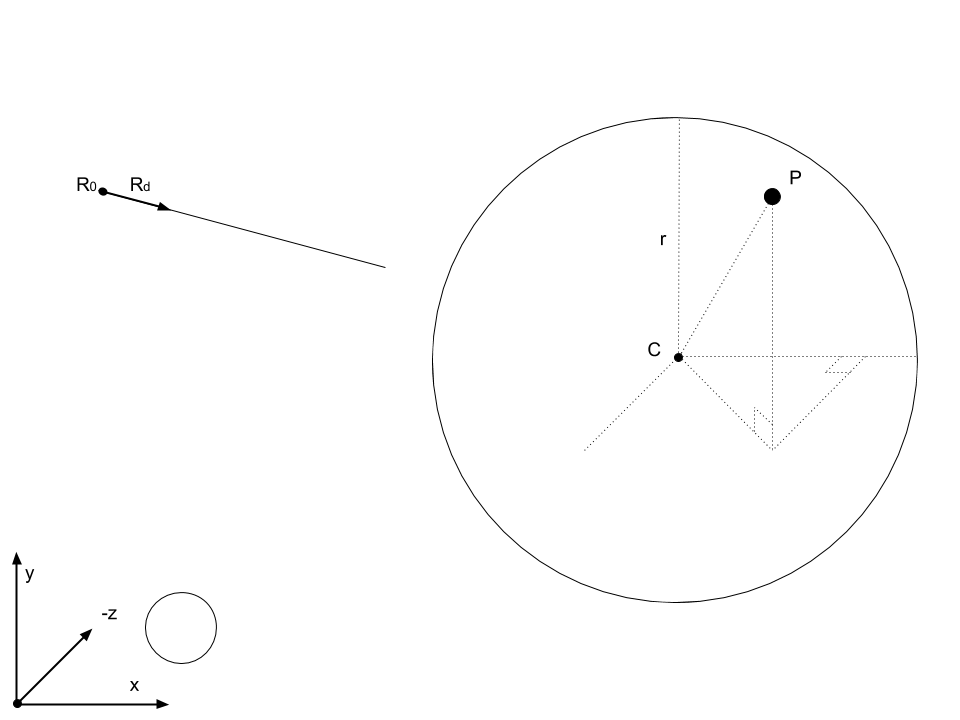
\includegraphics[width=\linewidth]{Figures/ray-sphere-intersection.png}
\decoRule
\caption[ray-sphere-intersection]{Ray-Sphere intersection}
\end{figure}

With known radius and center position, any point on the surface of sphere should match the equation:

\begin{equation}\label{equ:sphere-surface}
(x_{s} - x_{c})^2 + (y_{s} - y_{c})^2 + (z_{s} - z_{c})^2 = r^2
\end{equation}

If the ray intersects with the sphere, the intersection position must match the equation  \ref{equ:ray-t} and \ref{equ:sphere-surface}. Therefor the solution of \emph{t} in the cointegrate equation implies whether or not the ray will intersect with the sphere:

\begin{equation}\label{equ:ray-sphere}
\begin{aligned}
(x_{R_{0}} + x_{R_{d}} \cdot t - x_{c})^2 + (y_{R_{0}} + y_{R_{d}} \cdot t - y_{c})^2 + (z_{R_{0}} + z_{R_{d}} \cdot t - z_{c})^2 &= r^2 \\
&\vdots \\
x_{R_{d}}^2 \cdot t^2 + (2 \cdot x_{R_{d}} \cdot (x_{R_{0}} - x_{c})) \cdot t + (x_{R_{0}}^2 - 2 \cdot x_{R_{0}}\cdot x_{c} + x_{c}^2) & \\
+ y_{R_{d}}^2 \cdot t^2 + (2 \cdot y_{R_{d}} \cdot (y_{R_{0}} - y_{c})) \cdot t + (y_{R_{0}}^2 - 2 \cdot y_{R_{0}}\cdot y_{c} + y_{c}^2) & \\
+ z_{R_{d}}^2 \cdot t^2 + (2 \cdot z_{R_{d}} \cdot (z_{R_{0}} - z_{c})) \cdot t + (z_{R_{0}}^2 - 2 \cdot z_{R_{0}}\cdot z_{c} + z_{c}^2) &= r^2
\end{aligned}
\end{equation}

It can be seen as the quadratic formula:
\begin{equation}\label{equ:sphere-surface-quadratic-formula}
A \cdot t^2 + B \cdot t + C = 0
\end{equation}



%\begin{equation}\label{equ:sphere-surface-quadratic-formula}
%\begin{aligned}
%& A \cdot t^2 + B \cdot t + C = 0 \\
%& A = x_{R_{d}}^2 + y_{R_{d}}^2 + z_{R_{d}}^2 \\
%& B = 2 \cdot (x_{R_{d}} \cdot (x_{R_{0}} - x_{c}) + y_{R_{d}} \cdot (y_{R_{0}} - y_{c}) + z_{R_{d}} \cdot (z_{R_{0}} - z_{c})) \\
%& C = (x_{R_{0}} - x_{c})^2 + (y_{R_{0}} - y_{c})^2 + (z_{R_{0}} - z_{c})^2 - r^2
%\end{aligned}
%\end{equation}



%****************************************************************
\section{Section 2}
asdasd

\subsection{Subsection 1}
asdasdasd

\subsection{Subsection 2}
asdasdasdasd

%****************************************************************
\section{Section 3}

\subsection{Subsection 1}
asdasdasd

\subsection{Subsection 2}
asdasdasdasd

\subsection{Subsection 3}
asdasdasd

%****************************************************************
\section{Section 4}

